\documentclass[11pt]{article}

%------------------------------------------------------------------
%------------------------------------------------------------------
%------------------------------------------------------------------
% Informació de l'informe

\newcommand{\titol}{
	 Instrucciones para la realización de informes técnicos y científicos
	 }

\newcommand{\titolcap}{Instrucciones para la realización de informes}

\newcommand{\AlumnoA}{Alumno/a 1}
\newcommand{\AlumnoB}{Alumno/a 2}
\newcommand{\AlumnoC}{Alumno/a 3}

\newcommand{\AlumnosPie}{\AlumnoA\ -- \AlumnoB\ -- \AlumnoC}
\newcommand{\Asignatura}{Asignatura}
\newcommand{\CursoTitulacion}{4$.\!^\circ$ curso - Grado en Ingeniería ...}
%https://www.rae.es/dpd/ordinales

\newcommand{\Data}{Octubre de 2022}

%------------------------------------------------------------------
% Configuració de formats i bibliografia


\usepackage[spanish,es-tabla,es-nosectiondot,es-sloppy,es-noshorthands]{babel} 

\usepackage[utf8]{inputenc}
\usepackage{mathtools}
\usepackage{graphicx,xcolor}
\usepackage{tabularx,booktabs}

\usepackage{float}

\floatstyle{plaintop}
%\floatstyle{ruled}
\newfloat{listado}{htbp}{lol}
\floatname{listado}{Listado}

\usepackage[tableposition=top]{caption}
\renewcommand{\captionlabelfont}{\bfseries\small}
\renewcommand{\captionfont}{\small\itshape}
%\captionsetup[table]{position=above}

\usepackage{enumitem}
\setlist{leftmargin=1.25cm}

\renewcommand{\labelenumi}{\arabic{enumi})}
\renewcommand{\labelenumii}{\alph{enumii})}

% ---------------------------------------------------------------------
% Document electrònic

\usepackage[ 
    colorlinks,
    linkcolor = blue,
    urlcolor = blue,
    citecolor = blue,
    ]{hyperref}

% ---------------------------------------------------------------------
% Configuració de pàgina

\usepackage{geometry}
\geometry{
    a4paper, 
    twoside = false,
    hmargin = {2.5cm,2.5cm},
    vmargin = {1cm,1cm},
    headsep = 1.0cm,
    footskip = 1.5cm,
    includehead, includefoot
    }
        
% ---------------------------------------------------------------------
% Unitats del sistema internacional

\usepackage{siunitx}
\sisetup{
    output-decimal-marker = {,},
    % per-mode = symbol,
    }
    
% ---------------------------------------------------------------------
% Capçaleres i peus de pàgina

\usepackage{fancyhdr}
\pagestyle{fancy}

\usepackage{lastpage}

\fancyhead{} 
% \fancyhead[L]{\footnotesize \sffamily \titolcap}
% \fancyhead[R]{\footnotesize \sffamily \nouppercase \leftmark}
\fancyfoot{} 
% \fancyfoot[R]{\sffamily\footnotesize\thepage/\pageref*{LastPage}}
\ifundef{\AlumnosPie}
	{
		\fancyfoot[L]{\sffamily\footnotesize Se debe configurar el nombre de los alumnos que aparece en el pie}
	}
	{
		\fancyfoot[L]{\sffamily\footnotesize\AlumnosPie}
	}
\renewcommand{\headrulewidth}{0.4pt}
\renewcommand{\footrulewidth}{0.4pt}

% ---------------------------------------------------------------------
% Confiuració de la bibliografia

\usepackage[
	url = false,
	style = apa,
	%style = ieee,
	hyperref = true,
	backref = true,
	]{biblatex}

\usepackage{csquotes}

% ---------------------------------------------------------------------
% On estan les figures? 

\graphicspath{
    {./figuras/}
    {./logos/}
    }

% ---------------------------------------------------------------------
% Informació de portada

\usepackage{xifthen}

\newboolean{LogoUPV}
\newboolean{LogoAlcoi}

\ifundef{\AlumnoB}{\newcommand{\AlumnoB}{}}{}
\ifundef{\AlumnoC}{\newcommand{\AlumnoC}{}}{}

\title{\Huge\bfseries%
	\vspace*{-1cm}
    \ifLogoAlcoi
	   
\includegraphics[width=6cm]{UPV_Campus_Alcoi}\\
    \else
        
\includegraphics[width=6cm]{UPV_horitzontal_color}\\
    \fi
    \vspace*{5cm}
    \titol
    \vspace*{3.5cm}
    ~
    }
    
\author{
    \AlumnoA\\[1ex]
    \AlumnoB\\[1ex]
	\AlumnoC\\[3.5cm]
  	\textbf{\Asignatura}\\[2ex]
  	\textbf{\CursoTitulacion}
    }
    
\date{\Data}

% ---------------------------------------------------------------------
% Format de paràgraf

\parindent = 0cm
\parskip = 2ex
\partopsep = -1ex

% ---------------------------------------------------------------------
% Control de línies orfes i vídues

\clubpenalty = 10000
\widowpenalty = 10000
\displaywidowpenalty = 10000

% ---------------------------------------------------------------------
% Comandaments personalitzats

\usepackage{xspace}

\newcommand{\matlab}{{\textsc{Matlab}}\xspace}
\newcommand{\simulink}{\textit{Simulink}\xspace}


% ---------------------------------------------------------------------
% Fi
\usepackage{listings}

\definecolor{Paper}{HTML}{F5F5F5}

% ---------------------------------------------------------------------
% ---------------------------------------------------------------------
% Matlab

\lstset{
	language = Matlab,
	basicstyle = \ttfamily\footnotesize,         
	identifierstyle = ,           
	commentstyle = \color[rgb]{0,.5,0},
	stringstyle = \color[rgb]{.7,.2,.7},
	tabsize = 4,
	showstringspaces = false,
	frame = single,
	rulecolor = \color[rgb]{0.3,0.3,0.3},
	framerule = 0.2pt,
	framesep = 9pt,
	xleftmargin = 9pt,
	xrightmargin = 9pt,		
	backgroundcolor = \color{Paper},
	morekeywords = {},
	keywordstyle = \color{blue},
	}


% ---------------------------------------------------------------------
% ---------------------------------------------------------------------
% C

%\lstset{
%	language = C,
%	basicstyle = \ttfamily\small,         
%	identifierstyle = ,           
%	commentstyle = \color[rgb]{.4,.4,.4},%\itshape,
%	stringstyle = \color[rgb]{0,.5,0},
%	tabsize = 4,
%	morekeywords = {},
%	keywordstyle = \color{blue},	
%	frame=single,
%	framesep = 9pt,
%	xleftmargin = 24pt,
%	xrightmargin = 16pt,		
%	backgroundcolor = \color{Paper},
%	numbers = left,                    
%	numbersep = 16pt,                   
%	numberstyle = \scriptsize\color[rgb]{.4,.4,.4}, 
%	rulecolor = \color{black},         
%	showspaces = false,                
%	showstringspaces = false,          
%	showtabs = false,        
%	}

% ---------------------------------------------------------------------
% ---------------------------------------------------------------------

\lstset{literate= % Para poder usar acentos
  {á}{{\'a}}1 {é}{{\'e}}1 {í}{{\'i}}1 {ó}{{\'o}}1 {ú}{{\'u}}1
  {Á}{{\'A}}1 {É}{{\'E}}1 {Í}{{\'I}}1 {Ó}{{\'O}}1 {Ú}{{\'U}}1
  {à}{{\`a}}1 {è}{{\`e}}1 {ì}{{\`i}}1 {ò}{{\`o}}1 {ù}{{\`u}}1
  {À}{{\`A}}1 {È}{{\'E}}1 {Ì}{{\`I}}1 {Ò}{{\`O}}1 {Ù}{{\`U}}1
  {ä}{{\"a}}1 {ë}{{\"e}}1 {ï}{{\"i}}1 {ö}{{\"o}}1 {ü}{{\"u}}1
  {Ä}{{\"A}}1 {Ë}{{\"E}}1 {Ï}{{\"I}}1 {Ö}{{\"O}}1 {Ü}{{\"U}}1
  {â}{{\^a}}1 {ê}{{\^e}}1 {î}{{\^i}}1 {ô}{{\^o}}1 {û}{{\^u}}1
  {Â}{{\^A}}1 {Ê}{{\^E}}1 {Î}{{\^I}}1 {Ô}{{\^O}}1 {Û}{{\^U}}1
  {Ã}{{\~A}}1 {ã}{{\~a}}1 {Õ}{{\~O}}1 {õ}{{\~o}}1
}

% Si vols utilitzar un tipus de lletra semblant a Arial, descomenta les dos línies següents:
% \usepackage{cmbright}
% \usepackage[OT1]{fontenc}

\bibliography{./configuraciones/referencias}

%------------------------------------------------------------------
% Logo:

\setboolean{LogoUPV}{false}
\setboolean{LogoAlcoi}{true}

%------------------------------------------------------------------
%------------------------------------------------------------------
%------------------------------------------------------------------

\begin{document}

% -------------------------------------
% -------------------------------------


\renewcommand{\itemautorefname}{punto}
\renewcommand{\sectionautorefname}{sección}
\renewcommand{\subsectionautorefname}{subsección}
\renewcommand{\subsubsectionautorefname}{subsección}
\renewcommand{\appendixautorefname}{apéndice}
\renewcommand{\figureautorefname}{figura}
\renewcommand{\tableautorefname}{tabla}

\renewcommand{\indexname}{Índice alfabético}
\renewcommand{\bibname}{Bibliograf\'{\i}a}
\renewcommand{\contentsname}{Índice general}
\renewcommand{\abstractname}{Resumen}	

\def\listadoautorefname{listado}

% Per a les ecuacions en una línia
\abovedisplayshortskip = -1.0ex plus 0ex minus 0.25ex
\belowdisplayshortskip = 2.0ex plus 1ex minus 0.0ex

% Per a les equacions en varies línies
\abovedisplayskip = -1.0ex plus 0ex minus 0.25ex
\belowdisplayskip = 2.0ex plus 1ex minus 0.0ex

\begin{titlepage}
    \maketitle
    \thispagestyle{empty}
\end{titlepage}

\renewcommand{\thepage}{\Roman{page}}
\fancyfoot[R]{\sffamily\footnotesize\thepage}
\fancyhead{} 

\renewcommand{\headrulewidth}{0.0pt}

\setcounter{page}{1}

{
\footnotesize
\parskip=1ex

\tableofcontents

\clearpage

\listoffigures

\bigskip

\listoftables

}

\clearpage

\renewcommand{\thepage}{\arabic{page}}
\fancyfoot[R]{\sffamily\footnotesize\thepage/\pageref*{LastPage}}
\setcounter{page}{1}

\fancyhead[L]{\footnotesize \sffamily \titolcap}
\fancyhead[R]{\footnotesize \sffamily \nouppercase \leftmark}

\renewcommand{\headrulewidth}{0.4pt} % No eliminar!!!

% -------------------------------------
% -------------------------------------


%------------------------------------------------------------------
%------------------------------------------------------------------
% Resumen

\phantomsection
\addcontentsline{toc}{section}{Resumen}
\section*{Resumen}

Este documento es un pequeño manual para la realización de informes científico-técnicos y trabajos académicos. Se describe la estructura que debe tener un documento de este tipo y se describen las directrices estándar mínimas parar la redacción del contenido. También se incluyen recomendaciones para incluir figuras, tablas y ecuaciones, así como sobre la forma de hacer referencia a estos elementos en el documento. Por último, se incluyen ejemplos de figuras, tablas, ecuaciones y referencias bibliográficas.

Este documento también se puede utilizar como plantilla ya que los formatos son los adecuados para un documento científico-técnico.

\textbf{Palabras clave}: informe científico-técnico; plantilla; \LaTeX, Overleaf.

%------------------------------------------------------------------
%------------------------------------------------------------------

\section{Introducción}
\label{sec:introduccion}

Un informe científico-técnico es una descripción de los procedimientos, resultados obtenidos y conclusiones extraídas sobre un trabajo realizado por un equipo de científicos o técnicos. El objetivo último de un informe es comunicar a otros científicos u otros técnicos el trabajo realizado. Por lo tanto, un informe científico-técnico debe tener una estructura que permita su fácil comprensión y debe seguir unas normas en cuanto al contenido.

Este documento es una guía para la realización de informes científico-técnicos y trabajos académicos. En la \autoref{sec:estructura} se describe la estructura de este tipo de documentos y en la \autoref{sec:redaccion} se dan unas recomendaciones para afrontar la redacción de este tipo de documentos. En la \autoref{sec:contenido} se dan unas recomendaciones sobre el contenido del informe: estilo de redacción, figuras, tablas y ecuaciones. Por último, en la \autoref{sec:ejemplos} se proporcionan ejemplos de figuras, tablas, ecuaciones y referencias cruzadas a todos estos elementos.

%------------------------------------------------------------------
%------------------------------------------------------------------

\section{Estructura del informe}
\label{sec:estructura}

Los dos primeros elementos que se debe encontrar el lector en un documento son:

\begin{itemize}

    \item Una portada con el título del trabajo, los autores y la fecha. También es importante incluir información para enmarcar el trabajo, como asignatura, grado o máster etc.
    
    \item Una tabla de contenidos con todas las secciones y subsecciones del propio documento.
    
\end{itemize}

La estructura de un informe científico-técnico puede variar en función del objetivo del informe, pero siempre debe contener estos elementos:

\begin{enumerate} \itemsep = 0ex % Hemos modificado la distancia entre ítems
    \item Resumen y palabras clave
    \item Introducción
    \item Metodología
    \item Resultados
    \item Conclusiones y futuros trabajos
    \item Bibliografía
\end{enumerate}

Esta estructura es flexible y se debe adaptar a cada documento en particular, añadiendo o modificando las secciones y subsecciones que se consideren oportunos. Por ejemplo, se podría considerar la inclusión de una sección en la que se describe la configuración de los distintos dispositivos utilizados en los ensayos experimentales, se hace una revisión de la literatura o se profundiza en el marco teórico. También se pueden incluir anexos al final del documento con información adicional.

%------------------------------------------------------------------
\subsection{Resumen y palabras clave}

El resumen no suele ir numerado como el resto de las secciones y debe tener una extensión máxima de 250 a 300 palabras. El resumen debe contener la siguiente información: qué problema se resuelve, cómo se ha resuelto y qué conclusiones más importantes se han extraído. El resumen no debe incluir referencias bibliográficas.

El resumen debe captar la atención del lector. Solo leyendo el resumen, el lector debe saber si este documento le interesa o no. Por otra parte, se debe escribir al final del proceso de creación del documento.

Las palabras clave son términos o frases cortas que ayudan a definir la temática del trabajo y que sirven para que éste pueda ser recuperado en una búsqueda de información. El número de palabras clave recomendado es de 6.

%------------------------------------------------------------------
\subsection{Introducción}

La introducción ha de responder a la pregunta de por qué se ha realizado el trabajo que se presenta y centrar el foco en el objetivo del trabajo. Si se trata de un trabajo científico se debe destacar en primer lugar el interés del tema y el problema que se aborda. Si se trata de un trabajo académico para una asignatura, se debe describir qué problema se han resuelto y qué soluciones se han propuesto. También se pueden introducir los conceptos matemáticos utilizados haciendo referencias bibliográficas, ver la \autoref{sec:estructura:bibliografia} ``\nameref{sec:estructura:bibliografia}''. 

En la introducción se pueden utilizar tantas subsecciones como sean necesarias (o ninguna, o más de una subsección), o incluso crear nuevas secciones al mismo nivel que la introducción, si el marco teórico así lo requiere.

Al final de la introducción se debe describir la estructura del resto del documento y el contenido de cada uno de las secciones haciendo referencia cruzada a ellas. Esto facilitará al lector la localización de los contenidos que le interesen.

%------------------------------------------------------------------
\subsection{Metodología}

La metodología debe ser una lista numerada de los pasos que has seguido para resolver el problema planteado en la introducción. Por ejemplo (solo es un ejemplo):

\begin{enumerate}
    \item Ensayo de lazo abierto.
    \item Cálculo de los parámetros estándar del PID.
    \item Ensayo en lazo cerrado del regulador PID estándar.
\end{enumerate}

Cada uno los elementos de la lista numerada se pueden ampliar si es necesario con listas numeradas anidadas. Si alguno de los puntos de la metodología requiere un desarrollo más detallado, se puede considerar la opción de crear una sección al mismo nivel que la metodología.

%------------------------------------------------------------------
\subsection{Resultados obtenidos}

La sección de resultados tendrá tantas subsecciones como elementos hay en la lista numerada de la metodología. De esta manera, el lector sabrá siempre qué resultados se le está presentando en el marco de la metodología descrita.

Siempre que sea posible, se deben comentar y analizar las expresiones matemáticas y resultados numéricos obtenidos, sobre todo si son resultados finales o resultados intermedios que convenga comentar por su importancia en el posterior desarrollo. En cuanto a los resultados proporcionados en forma de representación gráfica o tabla de datos, se debe comentar y analizar todos y cada uno de ellos. Frases como ``Se puede observar que...'', o ``Se puede comprobar en la figura...'' deben ser habituales en un informe.

%------------------------------------------------------------------
\subsection{Conclusiones y futuros trabajos}

Si se comentan cada uno de los resultados obtenidos en la sección de ``Resultados'', será muy fácil redactar las conclusiones del trabajo: se puede hacer una recopilación de todos los comentarios y conclusiones que se han ido escribiendo, y se añaden las conclusiones finales.

Por otra parte, se deben enunciar las mejoras y futuros trabajos que se pueden realizar a partir de los resultados obtenidos, indicando si ya se está trabajando en alguna línea.

%------------------------------------------------------------------
\subsection{Bibliografía}
\label{sec:estructura:bibliografia}

Todo trabajo científico-técnico parte del trabajos teóricos o prácticos realizados previamente. Por tanto, siempre deben aparecer citas a las referencias bibliográficas utilizadas. No se debe citar la Wikipedia, ni incluir figuras de esta web. No se deben citar webs que no sean de reconocido prestigio (IEEE, ISA, ELSEVIER, …). En la la \autoref{sec:estructura:bibliografia} ``\nameref{sec:estructura:bibliografia}'', se incluyen algunos ejemplos de citas bibliográficas.


%------------------------------------------------------------------
%------------------------------------------------------------------

\section{Cómo afrontar la redacción del informe}
\label{sec:redaccion}

Este apartado está basado en el artículo artículo: \href{https://www.elsevier.com/connect/11-steps-to-structuring-a-science-paper-editors-will-take-seriously}{\itshape 11 steps to structuring a science paper editors will take seriously} que \href{https://www.linkedin.com/in/angel-borja-yerro-1320b76a/?originalSubdomain=es}{Angel Borja} tiene publicado en la web de Elsevier.

Aunque la estructura del informe es la que se ha descrito en el apartado anterior, es conveniente redactar el contenido del informe siguiendo estos pasos:

\begin{enumerate} \itemsep = 0ex % Hemos modificado la distancia entre ítems
    \item Preparar las figuras y tablas. Es el reflejo del trabajo realizado.
    \item Escribir la metodología.
    \item Escribir los resultados y la discusión de los mismos.
    \item Escribir una conclusión clara.
    \item Escribir una introducción convincente.
    \item Escribir el Resumen.
    \item Redactar un título conciso y descriptivo.
    \item Seleccionar las palabras clave.
    \item Escribir las referencias bibliográficas.
\end{enumerate}


Es importante empezar por las figuras y las tablas porque son el reflejo más directo del trabajo realizado. Después se escribe la metodología utilizada para llegar a esos resultados, y posteriormente se escribe la discusión de esos resultados y una conclusión clara. Los siguiente es escribir una buena introducción y el resumen. Por último, se escribe el título, las palabras clave, y las referencias bibliográficas.

%------------------------------------------------------------------
%------------------------------------------------------------------

\section{Contenido del informe}
\label{sec:contenido}

En esta sección se proporcionan algunas recomendaciones generales sobre el formato, estilo de redacción, figuras, tablas, y también sobre las expresiones matemáticas.

La Universitat Politècnica de València ha desarrollado una serie de BiblioGuías entre las que se encuentra una con recursos para la elaboración del TFG. Uno de los apartados es “Cómo redactar”:

\texttt{\url{https://biblioguias.webs.upv.es/bg/index.php/es/como-redactar}}


%------------------------------------------------------------------
\subsection{Consideraciones generales}

Estas son algunas recomendaciones sobre el estilo de redacción y el formato en general:

\begin{enumerate}

    \item Cada párrafo debe ir desarrollando una idea o tema que vaya enlazando poco a poco con el objetivo y la motivación del trabajo. Los párrafos ha de tener suficiente entidad, es decir, al menos 6 líneas siempre que sea posible.
    
    \item Se debe redactar preferiblemente en impersonal, aunque en ocasiones se puede utilizar la primera persona del plural: ``En este trabajo se ha analizado...'', ``Hemos comprobado que el comportamiento...''.

    \item Los párrafos deben estar justificados. Esta característica ya está configurada en esta plantilla.

    \item Los títulos de las secciones, subsecciones, etc. no deben finalizar con un punto. 

    \item La numeración de las secciones y subsecciones no debe llevar punto final. Esta característica ya está configurada en esta plantilla.

    \item En una determinada sección, no debe haber nunca una única subsección. Si se incluye una subsección, se debe incluir más de una. Si no es posible, no se incluye ninguna.

    \item Todas las secciones y subsecciones debe contener al menos un párrafo de texto antes de incluir la primera subsección.

\end{enumerate}


%------------------------------------------------------------------
\subsection{Figuras y tablas}

Las figuras y las tablas son elementos muy importantes en un documento científico-técnico ya que presentan datos experimentales y representan gráficamente resultados obtenidos. También se suelen incluir gráficos que ayudan a la mejor comprensión del contenido del informe. Por tanto, estos elementos deben ser incluidos en el documento siguiendo unas normas:

\begin{enumerate}

    \item Las figuras y las tablas a lo largo de todo el documento han de presentar un aspecto uniforme con un tamaño adecuado y utilizando una paleta de colores suave y sin estridencias.

    \item Se debe elegir el conjunto mínimo de figuras que representen claramente los resultados que se quieren mostrar. Es decir, un documento no puede contener demasiadas figuras. Si fuera necesario proporcionar gran número de figuras, se pueden agrupar en un anexo intentando ajustar varias figuras en una página.

    \item Todas las figuras y todas las tablas deben tener asociado un ``título'' (``\textit{caption}'') en el que se realiza una descripción del contenido.

    \item El título de las figuras se coloca en la parte inferior y el rótulo debe ser ``Figura''.

    \item El título de las tablas se coloca en la parte superior y el rótulo debe ser ``Tabla''.
    
    \item Todas las figuras y todas las tablas que aparecen en el documento deben ser comentadas en el texto y a través de una referencia cruzada.
    
    \item La referencia a las figuras y las tablas en el texto se debe realizar antes de que aparezcan. Es decir, el párrafo en el que se habla por primera vez de una figura debe ser anterior a la propia aparición de la figura o tabla. Después de la aparición de la figura o la tabla también se puede hacer referencia a ella para destacar algún aspecto o compararla con otra.
    
    \item Se debe realizar siempre una referencia cruzada a la figura o a la tabla. No se debe utilizar expresiones como: ``En la siguiente figura...''. En su lugar se debe utilizar expresiones con referencias cruzadas: ``Como se puede ver en la \autoref{fig:control_PID}''.

    \item Si una figura o una tabla no es de elaboración propia, se debe citar la fuente, o la dirección web de la que se ha obtenido indicando la fecha de la consulta.
    
\end{enumerate}

%------------------------------------------------------------------
\subsection{Expresiones matemáticas y ecuaciones}

Debemos recordar que hay dos tipos de expresiones matemáticas o ecuaciones:

\begin{itemize}

    \item Ecuaciones en línea con el texto. por ejemplo, esta ecuación define la segunda ley de Newton: $F = m\,a$. Se trata de una ecuación, no es texto en cursiva, y además esta ecuación está en línea con el texto.
	
	\item Ecuaciones destacadas. Son ecuaciones que están solas en una línea y centradas. Cuando se va a hacer referencia a ellas posteriormente, se suelen numerar. En la \autoref{sec:ejemplos:ecuaciones} ``\nameref{sec:ejemplos:ecuaciones}'' se pueden encontrar algunos ejemplos de ecuaciones destacadas numeradas y no numeradas.
	
\end{itemize}

A continuación, se enumeran los aspectos más importantes relacionados con las expresiones matemáticas y ecuaciones:

\begin{enumerate}

    \item Las ecuaciones son ecuaciones. NUNCA, NUNCA son imágenes capturadas de la web o de otros documentos PDF, o escaneadas de libros. Recuerda que \LaTeX\ fue diseñado principalmente para escribir expresiones matemáticas.
    
    \item No es conveniente numerar todas las ecuaciones, solo se deben numerar aquellas a las que se va a hacer referencia cruzada o ecuaciones con mucha importancia.
	
    \item Al contrario que las figuras y las tablas, se debe hacer referencia cruzada a una ecuación después de que aparezca numerada en el texto, no antes.
	
    \item Las deducciones matemáticas no deben escribirse completas, solo los pasos más importantes. Es habitual escribir frases como: ``... y, sustituyendo la expresión de la velocidad (3.12) en la ecuación de la energía cinética (3.11) y simplificando, obtenemos la siguiente expresión: ...''. No es necesario escribir todos los pasos de la simplificación, aunque sí se puede indicar cómo se ha realizado en el texto.
	
    \item El símbolo de producto entre variables o entre cantidades NUNCA, NUNCA será el asterisco (`*'). Para representar el producto entre dos variables o entre dos cantidades se puede optar por:
    
    \begin{enumerate}
        \item $F=ma$
        \item $F=m\,a$
        \item $F=m \cdot a$
        \item $F=m \times a$
        \item $F=2 \cdot 5 \; \unit{\newton}$
    \end{enumerate}
    
    \item Expresión de las unidades de medida:

    \texttt{\url{https://www.boe.es/boe/dias/2010/02/18/pdfs/BOE-A-2010-2625.pdf}}

    Se trata de una corrección de errores y erratas del Real Decreto 2032/2009, de 30 de diciembre, por el que se establecen las unidades legales de medida (se incorpora el texto completo). En el \textbf{capítulo III} se indica \textbf{cómo se expresan las unidades de medida}.
	
	\item Uso de la coma o del punto como separador decimal:
	
    \texttt{\url{https://www.boe.es/boe/dias/2020/04/29/pdfs/BOE-A-2020-4707.pdf}}
    
    Modificaciones del Real Decreto 2032/2009, de 30 de diciembre, por el que se establecen las unidades legales de medida. Una modificación importante es que \textbf{se permite el punto o la coma} (preferiblemente la coma) \textbf{como separador decimal}.
	
	En esta plantilla se ha configurado el uso del separador decimal a través del paquete \texttt{siunitx} en el fichero ``\texttt{premabulo.tex}'' (hacia la línea 56)  que se encuentra en la carpeta ``\texttt{configuraciones}''. Característica que tú puedes cambiar:
	
	\verb|\sisetup{output-decimal-marker = {,}}|
	
	Ejemplos de expresiones correctas de cantidades y sus unidades de medida utilizando el paquete \texttt{siunitx}:
	
    \begin{enumerate}
        \item $v = \qty{2.34E-3}{\meter\per\second} = \qty[per-mode=symbol]{2.34E-3}{\meter\per\second}$
        \item $I = \qty{48}{\milli\ampere}$
        \item $R = \qty{2.2}{\kilo\ohm} = \qty{2.2E3}{\ohm}$
    \end{enumerate}
	
	\medskip
	
	Ejemplos de unidades de medida \textbf{mal} expresadas (inaceptable):
	\begin{enumerate}
	    \item $v = 24\mathrm{m/s}$ (debe haber un espacio de separación entre la cantidad y la unidad).
	    \item $I = 48\;mA$ (las unidades se escriben en perfil romano, no en itálico).
	\end{enumerate}

\end{enumerate}

%------------------------------------------------------------------
%------------------------------------------------------------------

\section{Ejemplos}
\label{sec:ejemplos}

En esta sección se proporcionan algunos ejemplos de figuras, tablas, ecuaciones numeradas y no numeradas y referencias cruzadas a cada uno de estos elementos. También se incluyen referencias bibliográficas y cómo se deben citar en el texto.

%------------------------------------------------------------------
\subsection{Figuras, tablas y referencias cruzadas}

En la \autoref{fig:mapa:respuesta} se muestran dos gráficas generadas con Matlab con dos \textit{subplots}. En este caso el título de la figura es único y se hace referencia a la parte izquierda y la parte derecha de la figura. Se debe observar que en este mismo párrafo se ha realizado una referencia cruzada a esa misma figura. Otro ejemplo de figura simple es el que se muestra en la \autoref{fig:control_PID}.

\begin{figure}[H]
    \bigskip % Para serparar la figura del párrafo anterior
	\centering
  	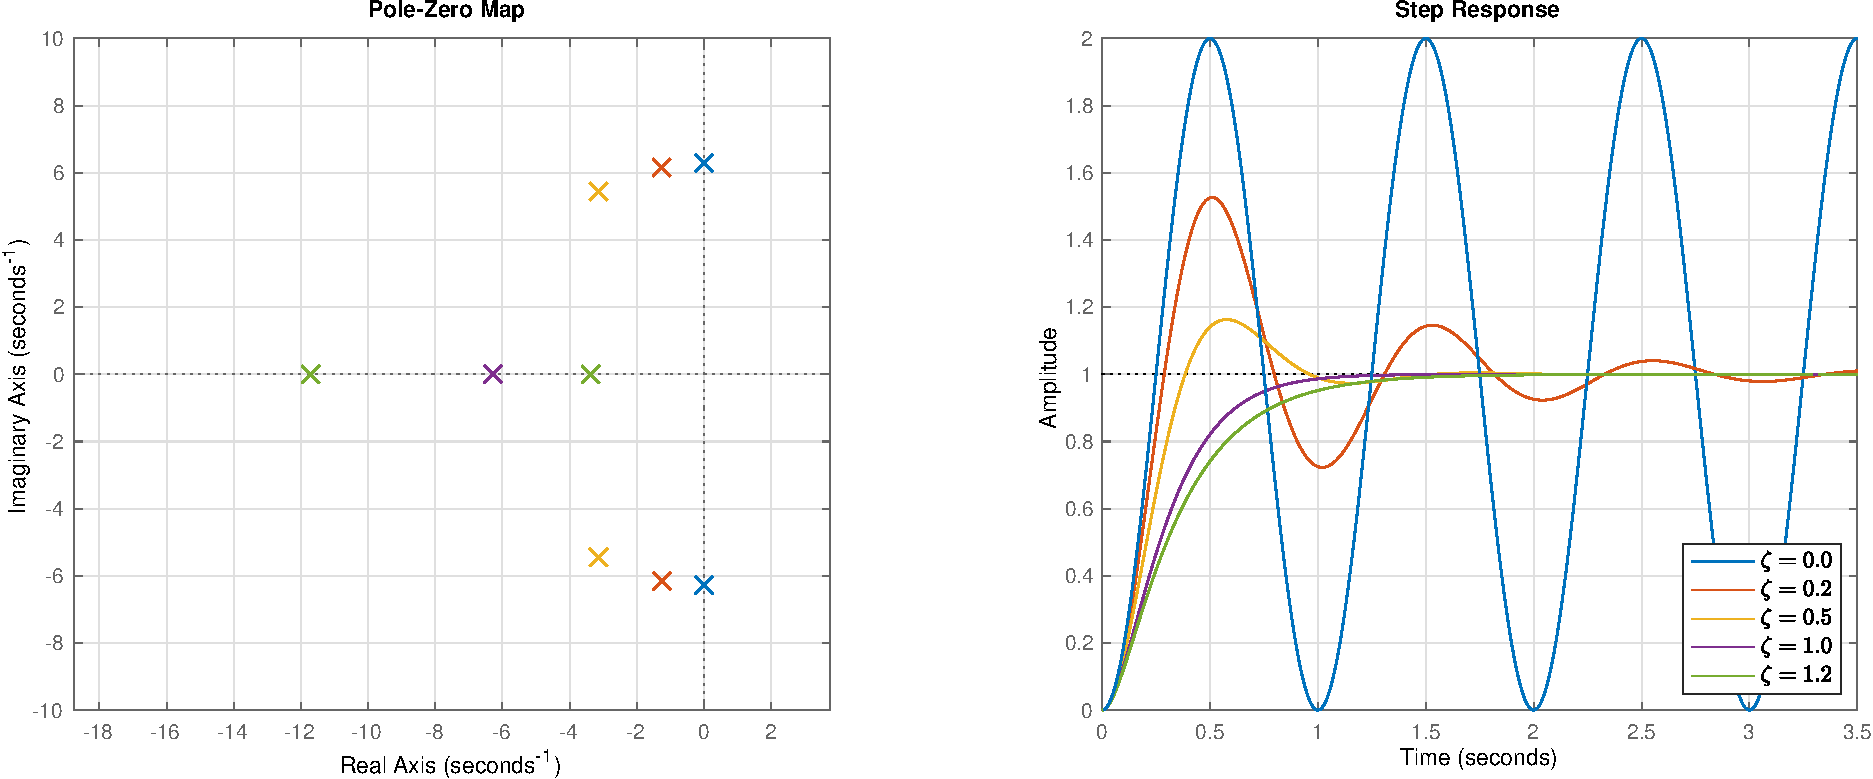
\includegraphics[width=\textwidth]{caracteritzaSegonOrdreZeta} % Figura en formato PDF
  	\caption{Mapa de polos y ceros (izquierda) y simulación en lazo cerrado (derecha)}
  	\label{fig:mapa:respuesta}
  	\medskip
\end{figure}

\begin{figure}[H]
	\centering
  	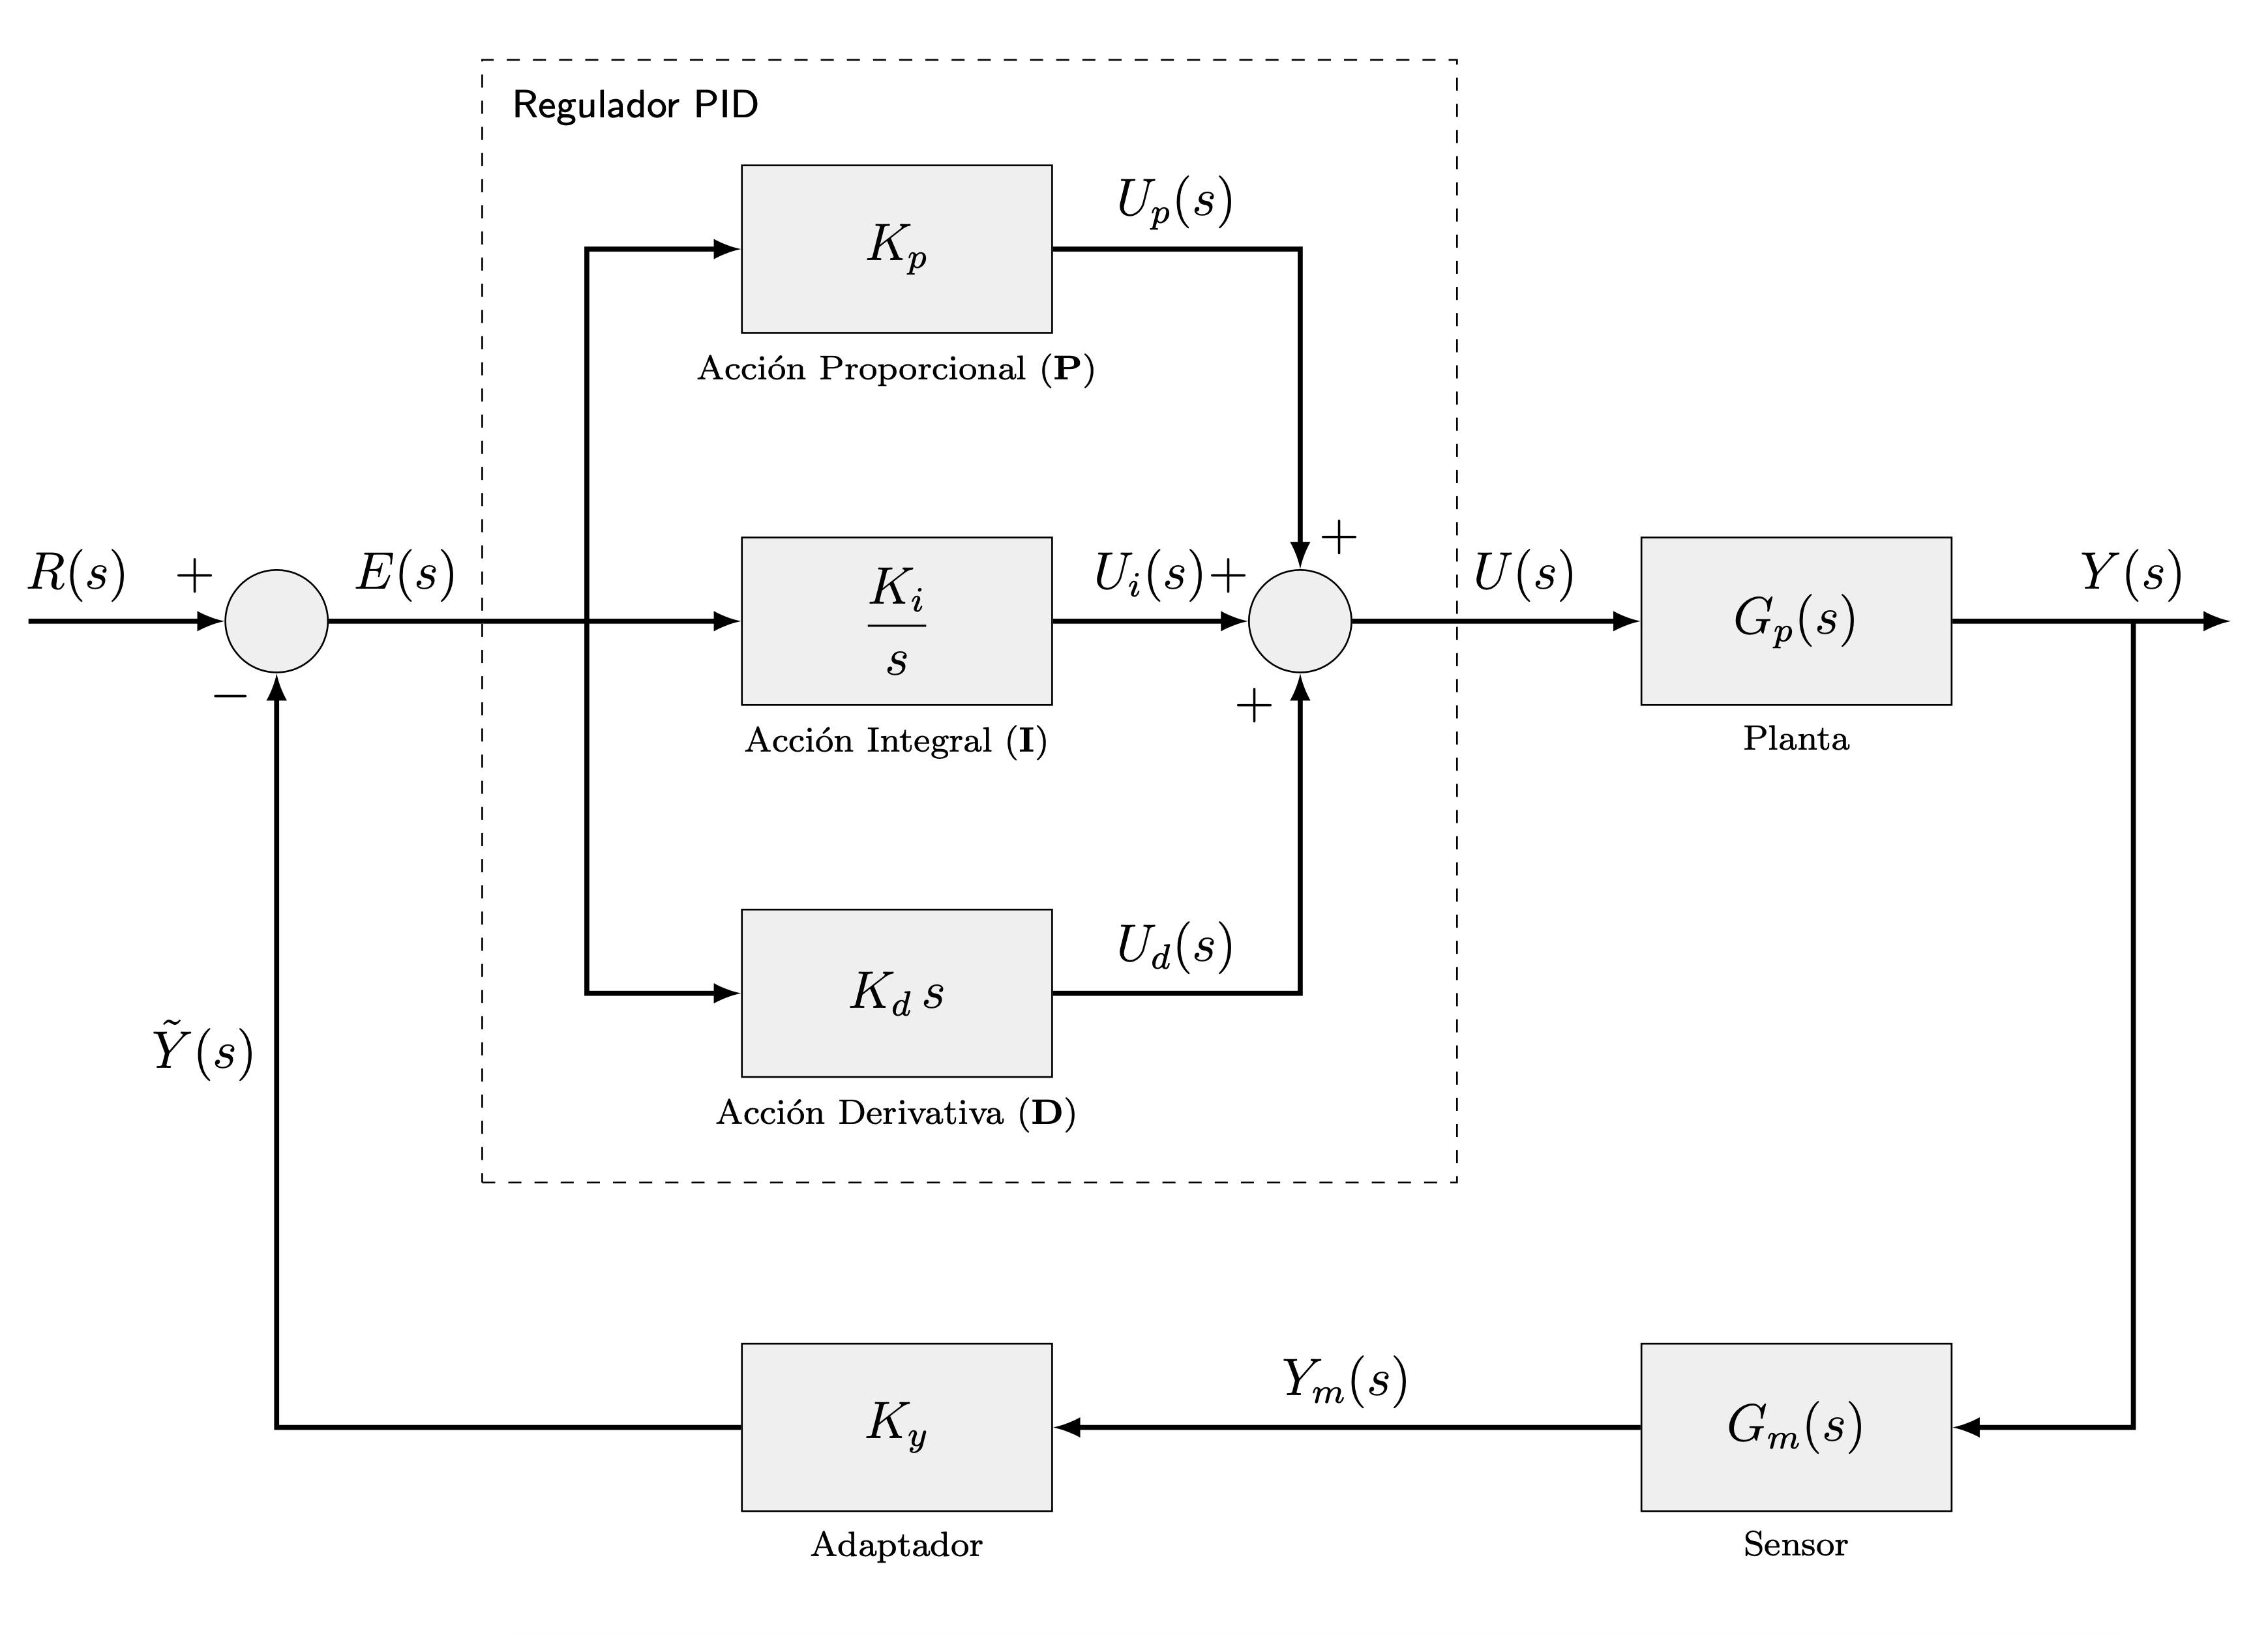
\includegraphics[width=.625\textwidth]{control_PID} % Figura en formato PNG
  	\captionsetup{width=0.625\textwidth} % Para conseguir que el título de la figura no sobrepase la figura
  	\caption{Diagrama de bloques detallado de un sistema controlado con un regulador PID}
  	\label{fig:control_PID}
\end{figure}

Pero hay casos en que interesa colocar dos figuras, una al lado de la otra, pero cada una con su propio epígrafe. Por ejemplo, la \autoref{fig:ldr-1} y la \autoref{fig:ldr-2} se encuentran una al lado de la otra, pero cada una tiene su propio título. En el código podrás ver el tipo de estructura que se ha utilizado para conseguir que las figuras se mantengan juntas. Por otra parte, puede ocurrir que estas dos figuras no estén inmediatamente después de este párrafo si no caben, pero esto no es problema porque se ha realizado una referencia cruzada a cada una de ellas.

\begin{figure}[ht]
    \centering
    \parbox[t]{0.475\textwidth}{\centering
    	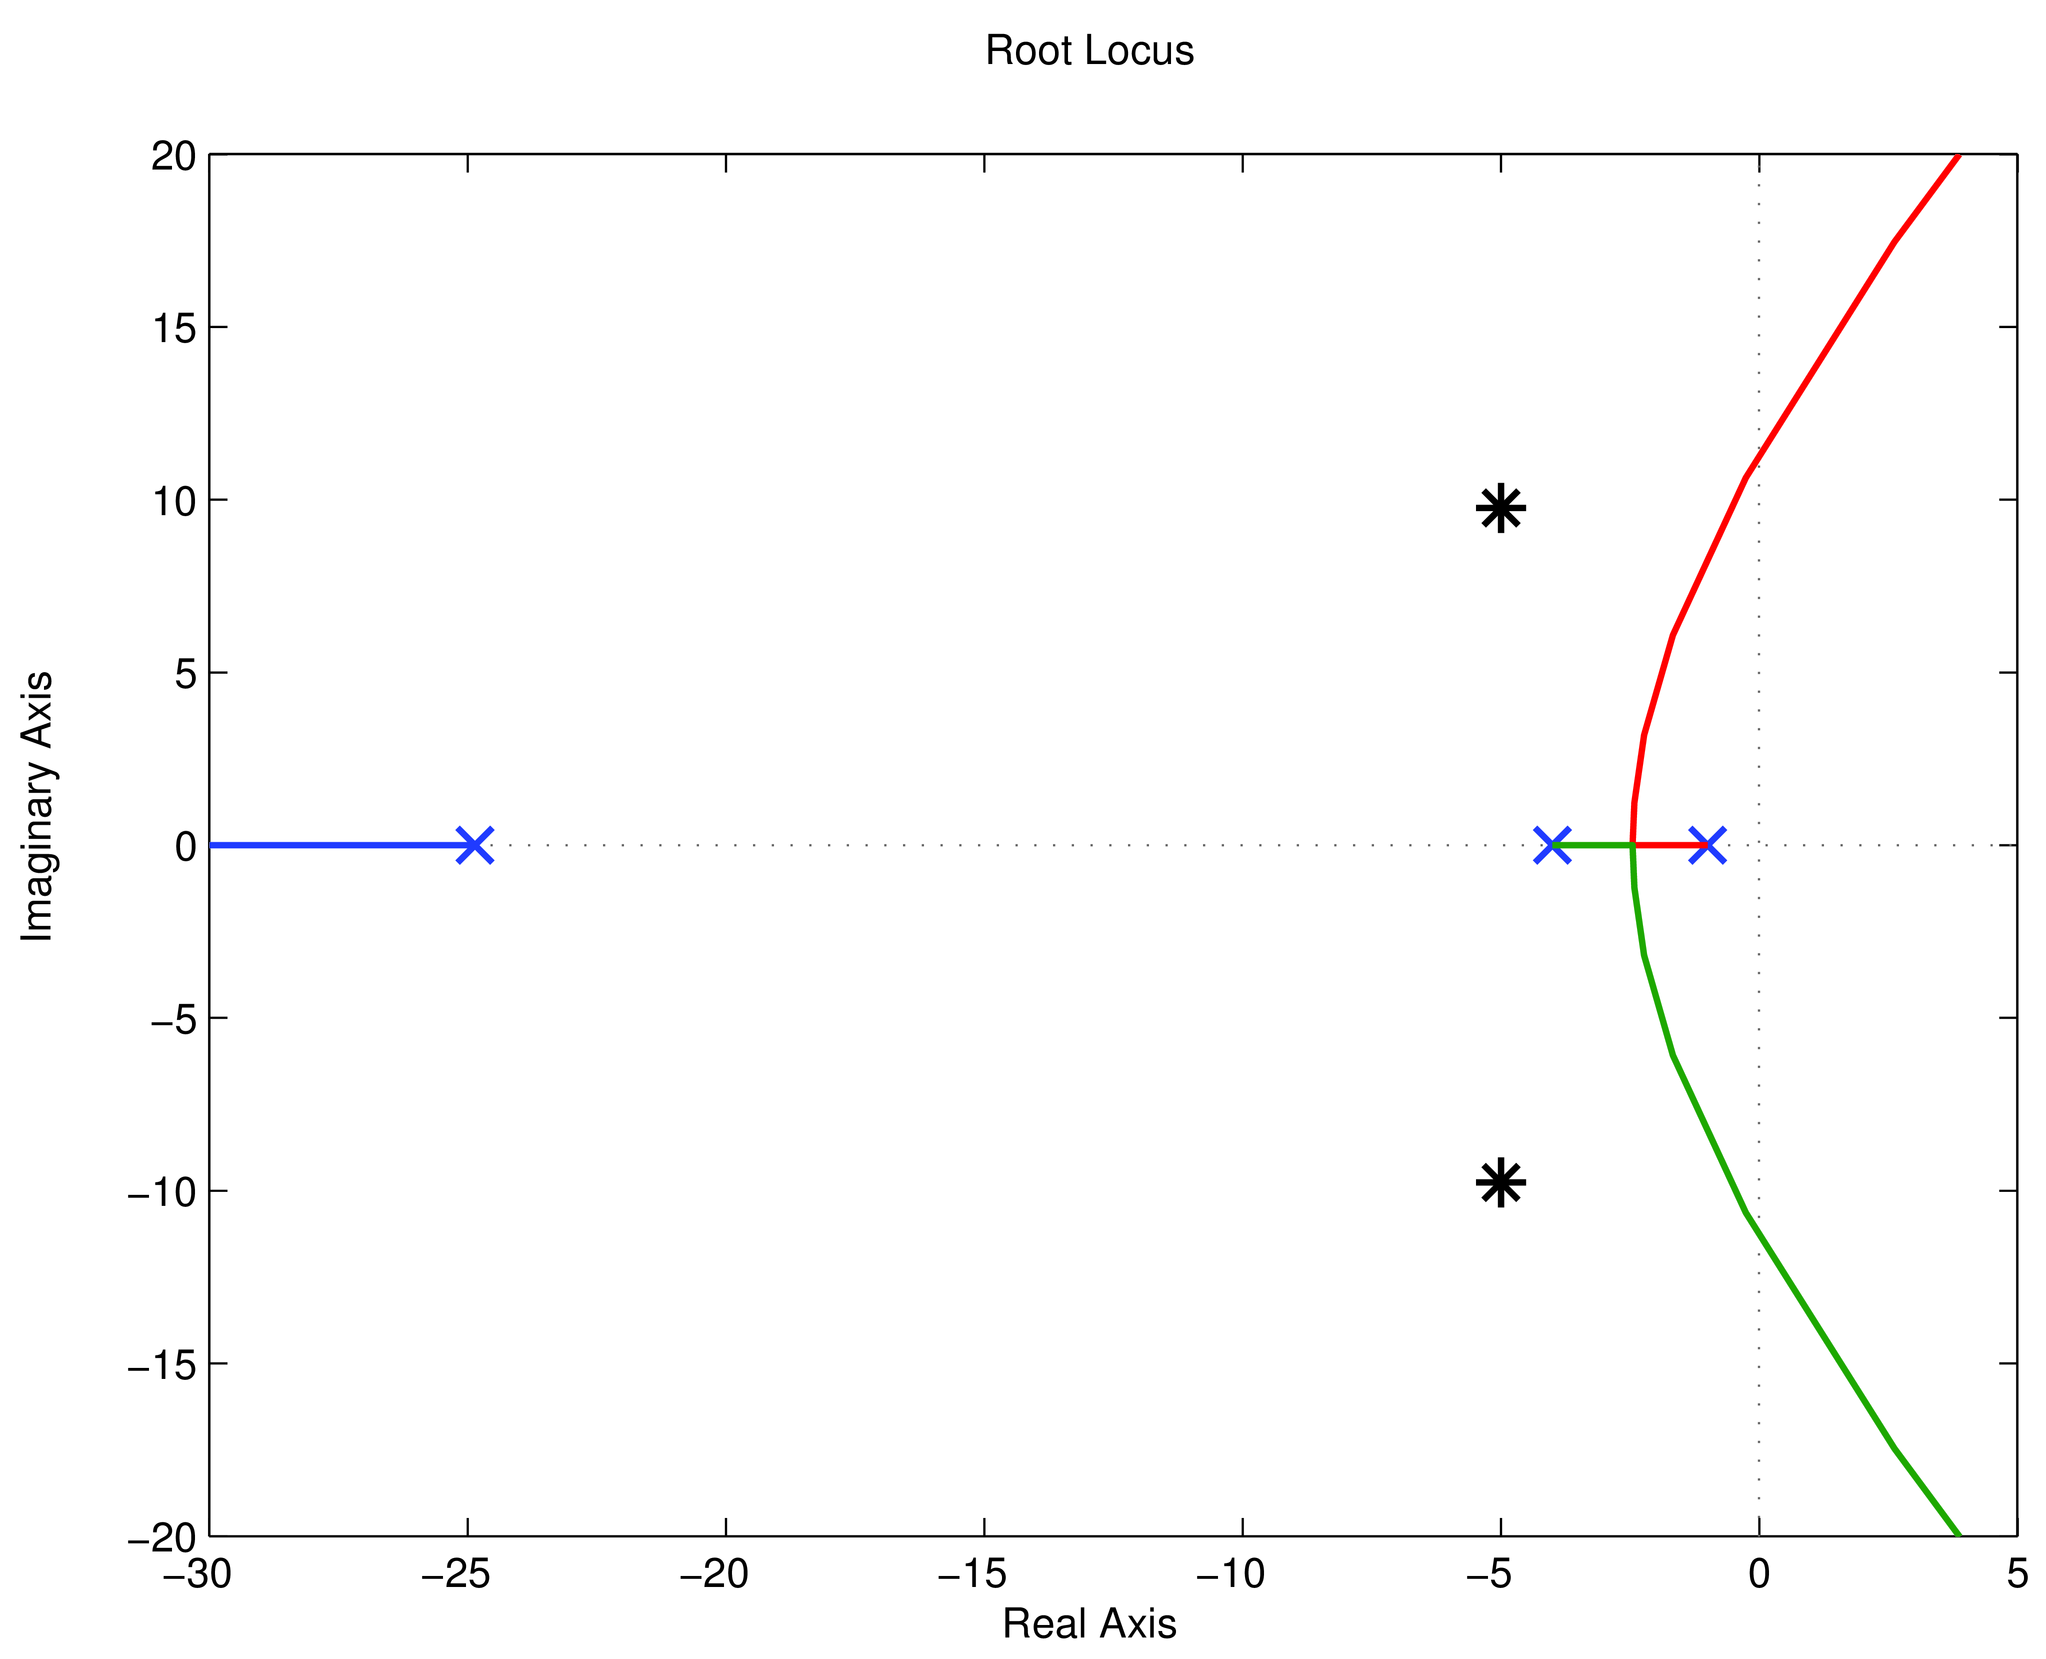
\includegraphics[width = 0.465\textwidth]{rl_sc2}
    	\captionof{figure}{Lugar de las raíces de la f.d.t. de lazo abierto modificada}
    	\label{fig:ldr-1}
    }
    \hfill
    \parbox[t]{0.475\textwidth}{\centering
    	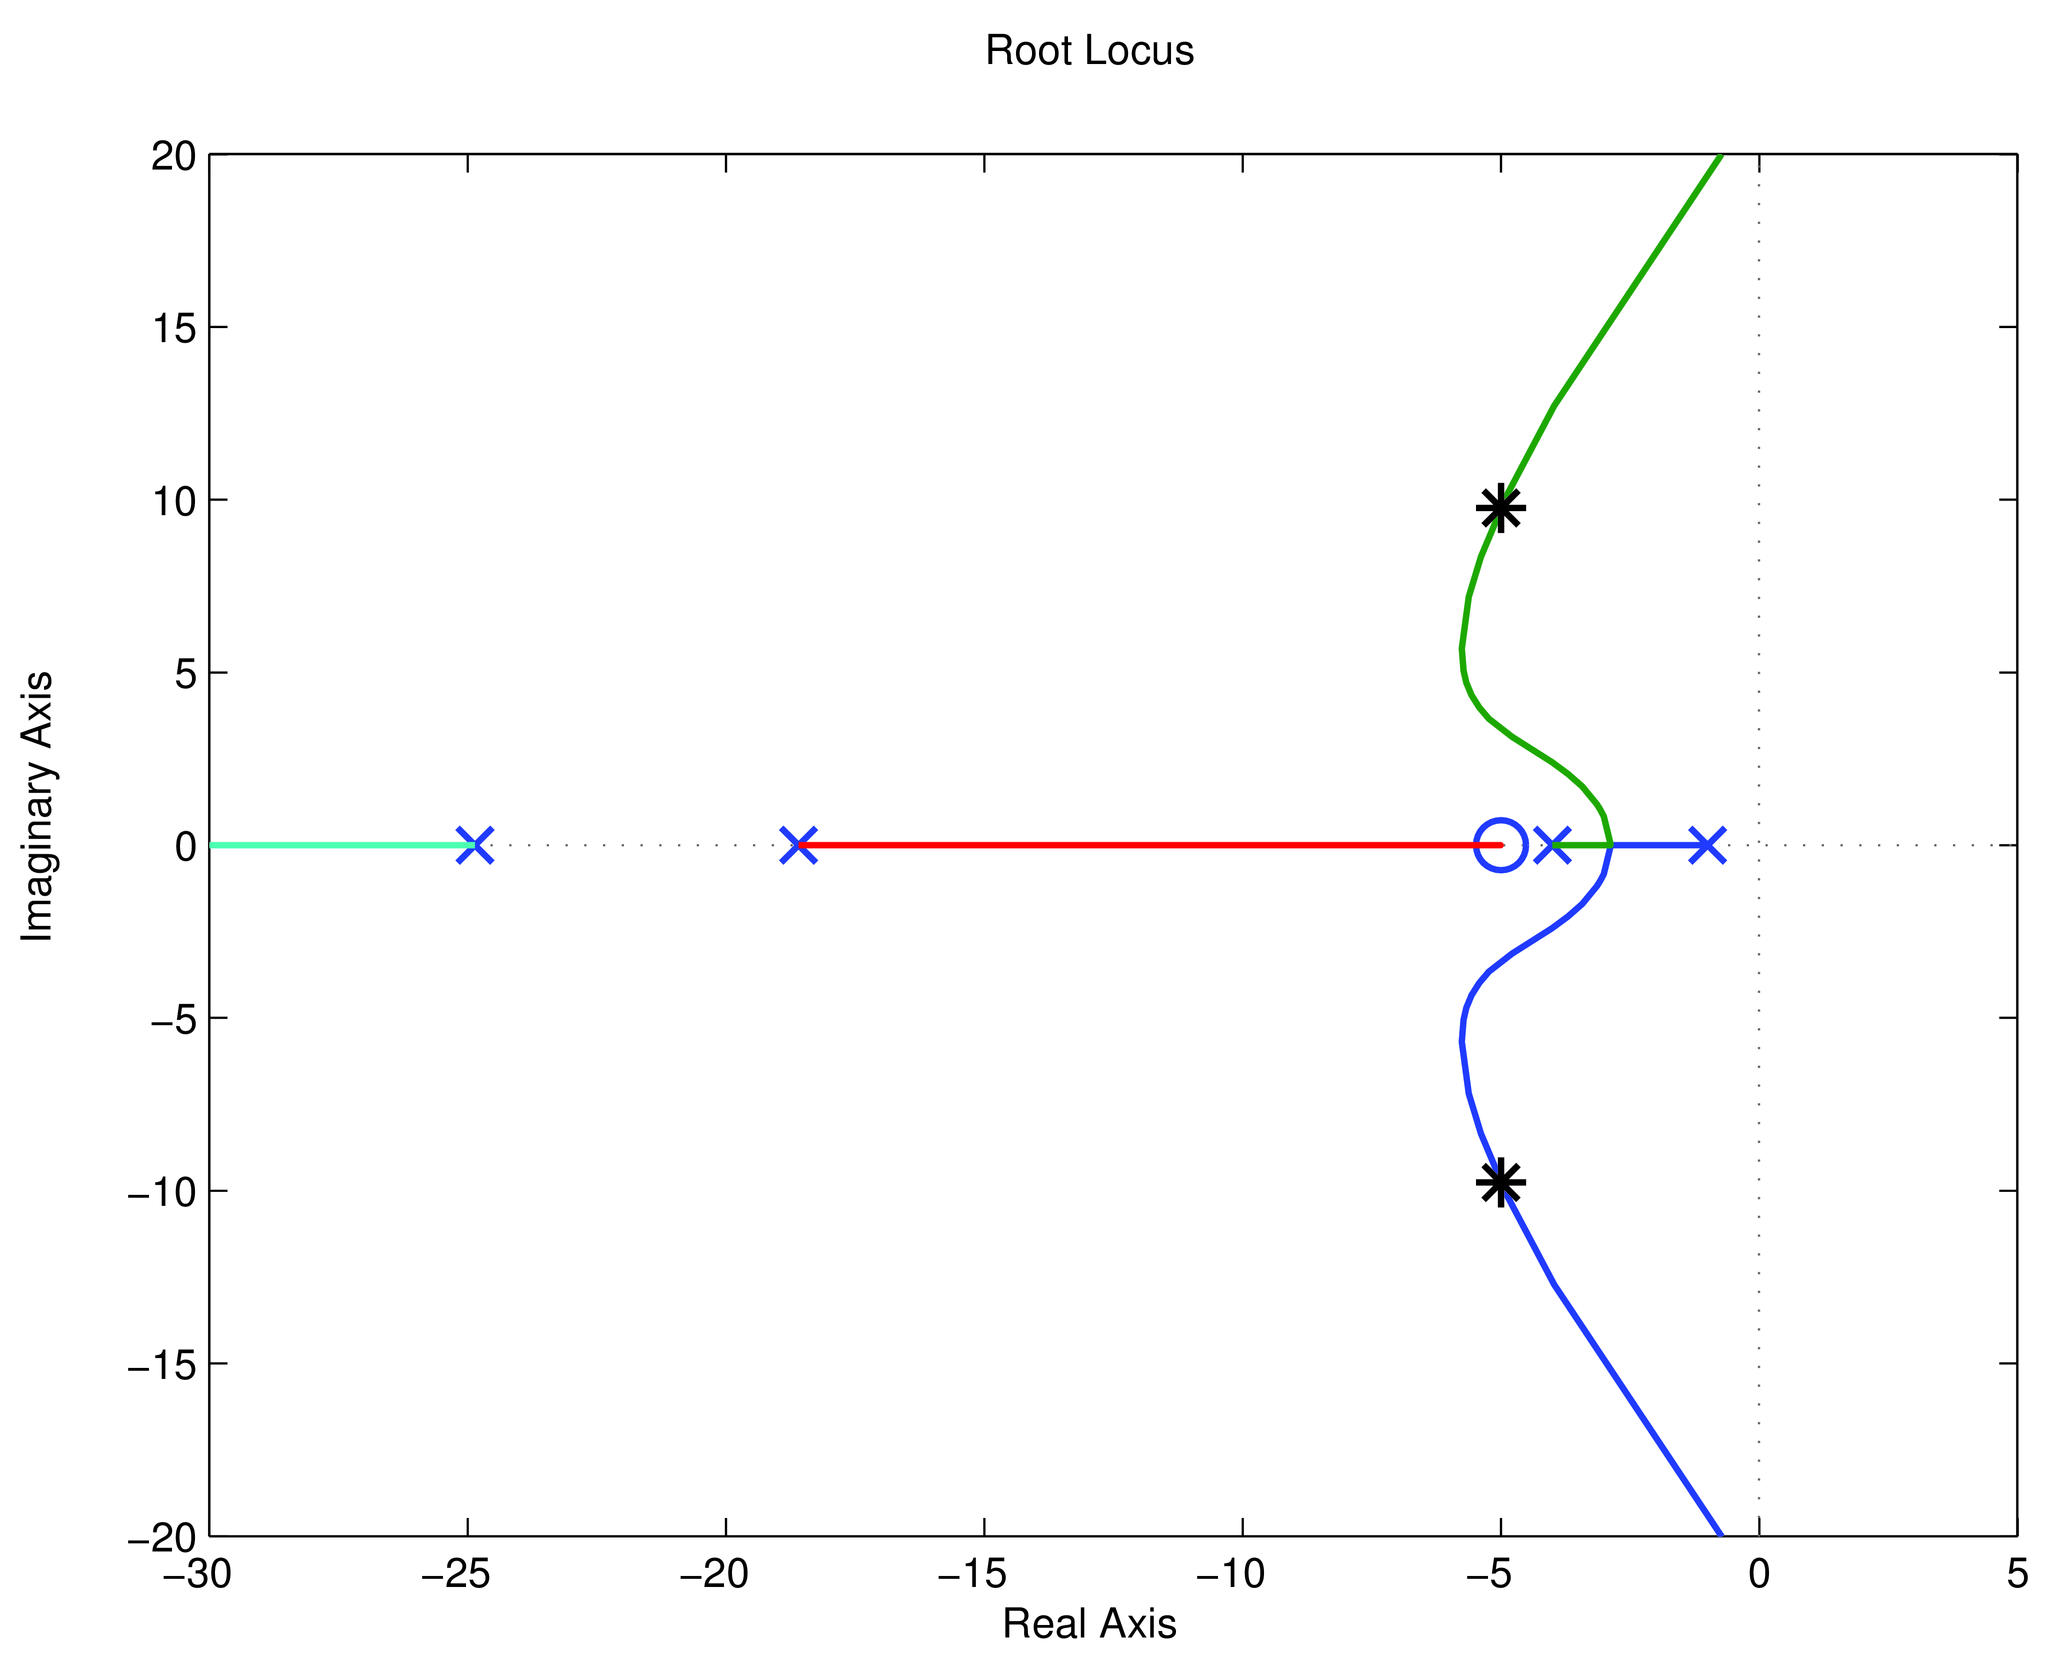
\includegraphics[width = 0.465\textwidth]{rl_c}
    	\captionof{figure}{Lugar de las raíces del sistema compensado}
    	\label{fig:ldr-2}
    }
\end{figure}

En la \autoref{tab:polos_SSO} se muestra la posición de los polos de un sistema de segundo orden en función del valor del coeficiente de amortiguamiento $\zeta$. Se puede observar que el título de la tabla se encuentra en la parte superior. Por otra parte, fíjate que hemos incluido expresiones matemáticas en línea con el texto en las celdas de la tabla.

\begin{table}[ht]
	\bigskip
	\centering

	\extrarowheight = -0.5ex
	\renewcommand{\arraystretch}{1.75}
	
	\captionsetup{width=0.7\textwidth}
	\caption{Polos de un sistema de segundo orden en función del coeficiente de amortiguamiento $\zeta$}
	\label{tab:polos_SSO}
	
	\begin{tabular}{ l l l }
	
	    \toprule
	    Condición
	    & 
	    Tipo de polos
	    & 
	    Posición de los polos: 
	    
	    \\ \midrule

	    $\zeta > 1$
        &
	    Reales simples
	    &
	    $s = -\zeta \omega_n \pm \omega_n \sqrt{\zeta^2 - 1}$

	    \\
	
	    $\zeta = 1$
	    &
		Real doble
	    &
	    $s = -\omega_n$ (doble)

	    \\
	
	    $0 < \zeta < 1$
	    &
	    Complejos conjugados
	    &
	    $s = -\zeta \omega_n \pm j\, \omega_n \sqrt{1 - \zeta^2}$

	    \\
	
	    $\zeta = 0$
	    &
	    Imaginarios puros
	    &
	    {$s = \pm j \, \omega_n$}

	    \\
	    
	    $\zeta < 0$
	    &
	    Parte real positiva
	    &
	    
        \\ \bottomrule
	
	\end{tabular}

	\bigskip

\end{table}


%------------------------------------------------------------------
\subsection{Ecuaciones}
\label{sec:ejemplos:ecuaciones}

No es conveniente numerar todas las expresiones matemáticas que aparecen en un documento. Como norma general, podemos numerar las ecuaciones a las que se va a hacer referencia cruzada, o aquellas que tengan una importancia clave en el desarrollo del trabajo. Un ejemplo de ecuación destacada no numerada es:

\begin{equation*} % Si incluimos el asterisco, no se numera la ecuación
    F = G\,\frac{m_1\,m_2}{r^2}
\end{equation*}

Por otra parte, en un documento \LaTeX\ es muy fácil numerar ecuaciones destacadas:

\begin{equation}\label{eqn:fdt}
    G(s) = \frac{1}{(RCs+1)}
\end{equation}
	
Recuerda que también existen las ecuaciones en línea con el texto, por ejemplo, la ecuación de un polinomio podrías ser $D(s) = (s+a)(s+b)$.

%------------------------------------------------------------------
\subsection{Código}

En muchas ocasiones es necesario incluir código en nuestro documento. Para ello definimos un elemento flotante nuevo (\texttt{listado}) y utilizamos el paquete \texttt{listings} que formatea de forma automática el código. En el \autoref{lst:EjemploMatlab} puedes ver el resultado final. Puedes cambiar el formato en el fichero ``\texttt{preambulo\_listings}'' que se encuentra en la carpeta ``\texttt{configuraciones}''.

\begin{listado}
\caption{Ejemplo de código Matlab}
\label{lst:EjemploMatlab}
\begin{lstlisting}
G = Gc*Gp;
H = Gm*Ky;
M = minreal(feedback(G,H)) polos_lc = pole(M);

figure(f2);
for i = 1 : length(polos_lc)
    if isreal(polos_lc(i))
        h = plot(polos_lc(i),0,'rx');
    else
        h = plot([polos_lc(i),polos_lc(i)'],'rx');
    end
    set(h,'LineWidth',0.75,'MarkerSize',16);
end

% Exportamos la figura en formato PNG
print(f2,'-dpng','-r300','LDR_cancela_04.png');
\end{lstlisting}
\end{listado}


%------------------------------------------------------------------
\subsection{Referencias bibliográficas}

Debemos distinguir entre la lista de referencias bibliográficas que se enumeran al final del documento, y las citas realizadas en el texto a estas referencias. Para realizar citas a referencias bibliográficas se puede hacer de forma explícita, por ejemplo ``... tal como se puede leer en \textcite{aastrom1973self}, y también en \textcite{ogata1996}'', o también entre paréntesis, \enquote*{La ingeniería de control es una pieza clave del desarrollo tecnológico \parencite{phillips1995}}.
% Fíjate que en esta última frase se ha utilizado el comando \enquote*{} para ponder comillas dobles.

Las referencias bibliográficas son el conjunto de libros, artículos y recursos web consultados para realizar el trabajo. Se organizan en forma de lista ordenada alfabéticamente por el apellido del primer autor. En la \autoref{sec:bibliografia} encontrarás cómo se imprimen las referencias.

%------------------------------------------------------------------
%------------------------------------------------------------------

\bibitemsep = 2ex
\bibhang = 2em

\printbibliography[heading=bibnumbered, title=\bibname, label=sec:bibliografia]

%------------------------------------------------------------------
%------------------------------------------------------------------
%------------------------------------------------------------------

\end{document}

%------------------------------------------------------------------
%------------------------------------------------------------------
%------------------------------------------------------------------

